\section{Experiments}
\subsection{Optimal solution verification}
In all cases, interface code was written so that the original author's code could be run without modification. Two methods were used to verify solution correctness: 1. manual visual verification of results for approximately 100 random graph pairs and 2. solution size verification against a second algorithm. The first method is used primarily as a sanity check on code integration. An example of the output MCS solution is below. 

\TODO{insert sample image of highlighted MCS mappings}

The second method follows the rationale that if multiple "optimal" search algorithms agree, then they are likely to be correct \cite{korf2014you}. We verify these results by using a second algorithm \cite{mccreesh2016clique} to solve the same MCS problem and compare the solution sizes. It should be noted that these algorithms output a single optimal mapping. As a result, while the mappings may differ between algorithms, the MCS size must be consistent to be correct. We use the author's original implementation and verify that for all three datasets (AIDS, LINUX, and IMDB), that the two solutions sizes are consistent.

\subsection{Baseline output stats}
Since we would like to train a network to predict the MCS of two graphs, we need to quantify the limits of the current state of the art algorithms. Following existing methods to quantify solution speed \cite{hoffmann2018observations}, we look at the total number of graphs that can be optimally solved in a given time limit, as a function of average graph size.

For small graphs (the AIDS and LINUX datasets), the MCSPLIT algorithm solves all instances in less than 1 second. Therefore, we analyze the IMDB dataset, setting a time limit of 1 minute for every solution. Figure \ref{fig:solution_limits} shows the percent of graph pairs solved as the average node count increases. 

\begin{figure}
    \centering
    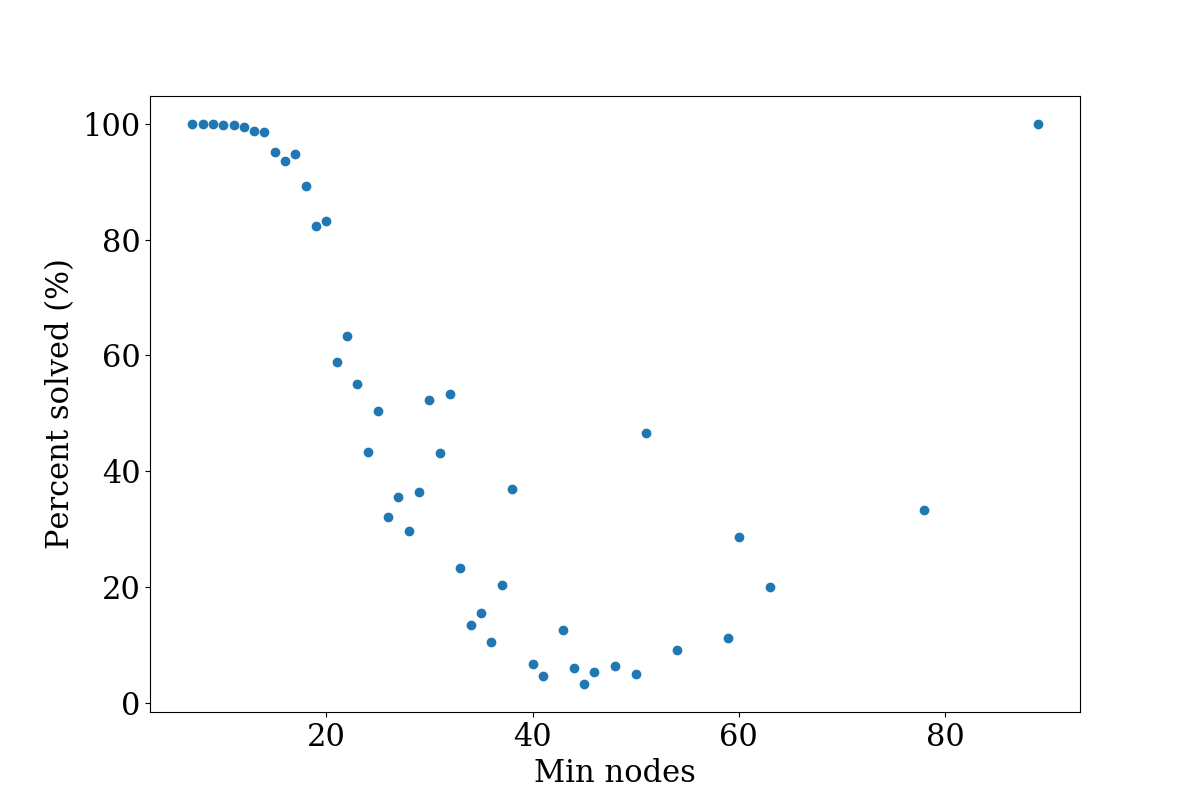
\includegraphics[width=\textwidth]{figures/pct_solved_avg_nodes.png}
    \caption{}
    \label{fig:solution_limits}
\end{figure}

\TODO{fix the graph}

\TODO{average mcs statistics (what is avg size of graphs and mcs size)}

\subsection{Trained AAAI model and results}


Following the results in \cite{bai2018convolutional}, we evaluate the model on the task of similarity search, where the similarity metric is the nMCS. We use mean squared error (mse), Kendall's Rank Correlation Coefficient $\tau$ \cite{kendall1938new}, Spearman's Rank Correlation Coefficient $\rho$ \cite{spearman1904proof}, and Precision at k (p@k) to evaluate the model. Rather than develop a new model to specifically learn the MCS problem, this work is focused on showing that MCS is a reasonable metric for similarity search and is learnable with an existing model.


- include the standard plot results

- include some sample ranking results

